% $Id: $
\documentclass[a4paper, 10pt]{article}
% reduced margins
\usepackage{fullpage}
\usepackage[authoryear]{natbib}
% spacing
\usepackage{setspace}
% page headings
\usepackage{fancyhdr}
%\usepackage{lscape}

\usepackage[nomain,acronym,xindy,toc]{glossaries} % nomain, if you define glossaries in a file, and you use \include{INP-00-glossary}
\makeglossaries

\usepackage[margin=1.0in]{geometry}
\usepackage{url}
%\usepackage{subeqn}
\usepackage{multirow}
\usepackage{booktabs}
\usepackage{enumerate}

\setlength{\headheight}{15.2pt}
\pagestyle{fancy}
% urls

\usepackage{lscape}
\usepackage{graphicx}
\usepackage{color}
\usepackage{hyperref}
\usepackage{url}
\hypersetup{colorlinks, urlcolor=darkblue}


\usepackage{lscape}
% figs to be 75% of test width
\setkeys{Gin}{width=0.75\textwidth}


%
\renewcommand{\abstractname}{\large SUMMARY}
%
\newcommand{\Keywords}[1]{\begin{center}\par\noindent{{\em KEYWORDS\/}: #1}\end{center}}
%
\makeatletter
\renewcommand{\subsubsection}{\@startsection{subsubsection}{3}{\z@}%
  {-1.25ex\@plus -1ex \@minus -.2ex}%
  {1.5ex \@plus .2ex}%
  {\normalfont\slshape}}
\renewcommand{\subsection}{\@startsection{subsection}{2}{\z@}%
  {-3.25ex\@plus -1ex \@minus -.2ex}%
  {1.5ex \@plus .2ex}%
  {\normalfont\bfseries\slshape}}
\renewcommand{\section}{\@startsection{section}{1}{\z@}%
  {-5.25ex\@plus -1ex \@minus -.2ex}%
  {1.5ex \@plus .2ex}%
  {\normalfont\bfseries}}
\makeatother
%
\renewcommand\thesection{\arabic{section}.}
\renewcommand\thesubsection{\thesection\arabic{subsection}}
\renewcommand\thesubsubsection{\thesubsection\arabic{subsubsection}}
%
\renewcommand{\headrulewidth}{0pt}

\usepackage{listings}

\newenvironment{mylisting}
{\begin{list}{}{\setlength{\leftmargin}{1em}}\item\scriptsize\bfseries}
{\end{list}}

\newenvironment{mytinylisting}
{\begin{list}{}{\setlength{\leftmargin}{1em}}\item\tiny\bfseries}
{\end{list}}

\usepackage{listings}

\definecolor{darkblue}{rgb}{0,0,0.5}
\definecolor{shadecolor}{rgb}{1,1,0.95}
\definecolor{shade}{rgb}{1,1,0.95}


\lstset{ %
language=R,   % the language of the code
basicstyle=\footnotesize, % the size of the fonts that are used for the code
numbers=left,   % where to put the line-numbers
numberstyle=\footnotesize, % the size of the fonts that are used for the line-numbers
stepnumber=1	00,   % the step between two line-numbers. If it's 1, each line 
    % will be numbered
numbersep=5pt,   % how far the line-numbers are from the code
backgroundcolor=\color{shade}, % choose the background color. You must add \usepackage{color}
showspaces=false,  % show spaces adding particular underscores
showstringspaces=false,  % underline spaces within strings
showtabs=false,   % show tabs within strings adding particular underscores
frame=single,   % adds a frame around the code
tabsize=2,   % sets default tabsize to 2 spaces
captionpos=b,   % sets the caption-position to bottom
breaklines=true,  % sets automatic line breaking
breakatwhitespace=false, % sets if automatic breaks should only happen at whitespace
title=\lstname,   % show the filename of files included with \lstinputlisting;
    % also try caption instead of title
escapeinside={\%*}{*)},  % if you want to add a comment within your code
morekeywords={*,...}  % if you want to add more keywords to the set
}

%
\title{Identification Of The Major Sensitivities In The East Atlantic And Mediterranean Bluefin Assessment}
%
\author{Laurence T. Kell\footnote{ICCAT Secretariat, C/Coraz\'{o}n de Mar\'{\i}a, 8. 28002 Madrid, Spain; ~Laurie.Kell@iccat.int; ~Phone: +34 914 165 600 ~Fax: +34 914 152 612.}
        }
 
%
\date{}
%
\begin{document}


\onehalfspacing
\lhead{\normalsize\textsf{SCRS/2014/020}}
\rhead{}

\maketitle
% gets headers on title page ...
\thispagestyle{fancy}
% ... but not on others
\pagestyle{empty}

%
\begin{abstract}

\textit{
Although several sources of uncertainty were considered when formulating the East Atlantic and 
Mediterranean Bluefin Tuna Recovery Plan, not all sources of uncertainty were explicitly 
considered in advice provided by the SCRS. This study uses a simple deterministic model to identify  
which sources of uncertainty have the biggest impact on advice and therefore which scenarios 
should be included in the Operating Model when conducting Management Strategy Evaluation.
}

\end{abstract}

\Keywords{Bluefin, Hypotheses, Management Strategy Evaluation, Operating Model, Sensitivity Analysis, Uncertainty}

 
\newpage
\tableofcontents
\newpage

\section{Introduction}

Although several sources of uncertainty were considered when formulating the East Atlantic and 
Mediterranean Bluefin Tuna Recovery Plan, not all sources of uncertainty were explicitly 
considered \citep{scrsbft2012}. Therefore a qualitative risk analysis was conducted in order to elicit from
stakeholder their main concerns with respect to uncertain \cite{leachrisk2013}.

The meeting on bluefin stock assessment methods \citep{scrsbftmethods2013} endorsed the work conducted so far on 
Risk Analysis and recommended that i) the major sensitivities for both separate and mixed stock assessments 
(e.g., M, fecundity schedule, SRR and alternative mechanism of population regulation) should be identified and 
ii) that a paper on a Risk Assessment be written to inform Operating Model (OM) scenarios to be
used in a Management Strategy Evaluation (MSE) based on the qualitative identification 
of uncertainty. 

In this study we develop a simple deterministic model that allows the impact of model and value uncertainty on stock 
assessment advice to be evaluated. The approach is intended to identify the single stock (i.e. excluding mixing) 
scenarios to be included in the Operating Model (OM) used in the bluefin Management Strategy Evaluation (MSE).
Under the GBYP methods for turning the qualitative risk analysis into a quantitative one have been developed 
\cite{levontinrisk} which will use the work described in this paper to conduct a Risk Assessment to help inform 
OM scenarios to be used in the MSE. 

\section{Material and Methods}

When building an OM it is necessary to develop hypotheses about system dynamics that can be
run as part of stochastic Monte Carlo simulations. However, Monte Carlo simulations are costly 
in time and resource to conduct. Therefore there are benefits in initially running deterministic 
(or a limited number of stochastic) of simulations to identify the most important effects or interactions. 
Following this fully stochastic simulations can be run for the trials (i.e. scenarios) that
are considered to be important. 

\subsection{Uncertainty}

Traditional stock assessments mainly considers only uncertainty in observations and process (e.g. recruitment). 
However, uncertainty about the actual dynamics (i.e. model uncertainty) has a larger impact on achieving management objectives \cite{punt_refocusing_2008}. 
Therefore when providing management advice it is important to consider appropriate sources of uncertainty.  \cite{rosenberg1994uncertainty} 
categorised uncertainties in fish stock 
assessment and management as:

\begin{itemize}
 \item Process error; caused by disregarding variability, temporal and spatial, in dynamic population and fisheries processes;
 \item Observation error;  sampling error and measurement error;
 \item Estimation error; arising when estimating parameters of the models used in the assessment procedure;
 \item Model error; related to the ability of the model structure to capture the core of the system dynamics;
 \item Implementation error;  where the effects of management actions may differ from those intended.
\end{itemize}

Sources of uncertainty related to \emph{Model Error} include
    
\begin{itemize}
 \item structural uncertainty; due to inadequate models, incomplete or competing conceptual frameworks, or where significant processes or 
relationships are wrongly specified or not considered. Such situations tend to be underestimated by experts \cite{morgan1990uncertainty}. and
 \item value uncertainty; due to missing or inaccurate data or poorly known parameters.
\end{itemize}

As part of the implementation of a management plan uncertainty related to how results are used also need to be considered \cite{francis54c} and 
include 

\begin{itemize}
 \item translational uncertainty; in explaining uncertain results and 
 \item institutional uncertainty; due to lack of social capital (i.e. ways to handle these types of problems) in stakeholder organisations 
to cope with management issues. 
\end{itemize}

Here we only deal with model and value uncertainty.

\subsection{Life-history}

Life-history traits are taken from the last SCRS assessment and are described in \cite{kell2012evaluation} i.e.

\begin{itemize}
 \item annual spawning (1 cohort per year), 
50\% maturity at age 4, 100\% maturity at ages 5+, 
 \item fecundity is linearly proportional to weight, 
 \item growth follows the von-Bertalanffy equation used in the ICCAT working group (with the following parameters: $L_{\infty}$ = 318.85, k=0.093, tO=-0.97), 
 \item length-weight relationship used in the ICCAT working group (W=2.95.10-5*L2.899),
 \item lifespan of 40 years.
 \item age-specific, but time-invariant, natural mortality based on tagging experiments on the southern bluefin tuna and used 
 in the ICCAT working group (i.e. M=0.49 for age 1, M=0.24 for ages 2 to 5, M=0.2 for age 6, M=0.175 for age 7, M=0.15 for 
 age 8, M=0.125 for age 9 and M=0.1 for ages 10 to 20).
\end{itemize}

\subsection{Model}

Given the selection pattern (s) of a fishery, and the catchability (q) of a population for a given effort (E), the fishing mortality rate 
($F_{a,y,j}$) for age a, year y, and population j is given by:

\begin{equation}F_{a,y,j} = E_y*q_j*s_{a,j} \end{equation}

Catchability, q, is assumed to be constant across age and time.
The selectivity pattern (sa) is assumed to vary by age .
The abundance ($N_j$) at age a+1, at the start of year y+1, in sub-population j, is:

\begin{equation}N_{a+1,y+1,j} = N_{a,y,j}*exp(-F_{a,y,j}- M_{a,y,j}) \end{equation}

In the assessment recruitment was assumed to be independent  of spawning stock biomass, i.e. recruitment is environmentally driven and steepness=1. 
We also consider the alternative  scenario that recruitment is dependent on S and follows a \cite{beverton_dynamics_1993} stock recruitment relationship with 
fixed parameters $\alpha$ and $\beta$ by arbitrarily assuming a value of steepness equal to 0.7. 
Virgin biomass of the population was estimated from the historic time series for each scenario 
for a given value of steepness, assuming a Beverton and Holt stock recruitment relationship.
 
\subsection{Scenarios}


\subsubsection{Factorial Design}

A full MSE requires appropriate uncertainty to be considered, particularly in the choice of OM scenarios. 
 
One way of doing this is base the choice of scenarios are based on a factorial design.  A full factorial experiment is one whose 
design consists of two or more factors, each with discrete possible values or \textit{levels}, and where experimental 
units take on all possible combinations of these levels across all factors. Such a design is better able to
represents the complexity of the real world and allows an evaluation of whether the effect of one factor
depends on the level of another factor. The potentially large number of combinations in a full factorial design 
may mean that it is not possible to run them all in the time available in a stock assessment working group.
Therefore a fractional factorial design in which some of the possible combinations are omitted may be preferred.

When conducting a Management Strategy Evaluation a large number of scenarios need to be considered to
evaluate the main sources of uncertainties. I.e. the OM will need to be 
conditioned on a wider range of data and knowledge that routinely considered within a stock assessment. 

In other words while only a few scenarios are routinely be considered within an ICCAT stock assessment, many more 
scenarios will need to be run as part of an MSE. This presents a potential problem if
the Scenarios from an MSE result in different conclusions from those ran in a stock assessment.

A base case be proposed and then factors with levels that represent the main uncertainties. In the
stock assessment WG the main effects can be evaluated by varying 1 factor at a time. Hopefully this will 
allow the stock assessment to \textit{bracket} the main uncertainty and act as a simple screening experiment, 
to determine the factors have the greatest influence on the perception of stock dynamics.
Based on the identification of the most important factors, a multi-level designed experiment can then be developed
for the MSE that includes interactions between factors.

The factors and levels in table \ref{tab:scn}. The $3_{rd}$ column summarises the 
number of levels for each factor. The $4_{th}$ column shows the cumulative number of scenarios if only the 
main effects are modelled, i.e. one a single level is varied in the base case at a time. The $5_{th}$ column 
shows the cumulative number of scenarios if all interactions between factors are considered.

The second block are scenarios that will be considered in other papers, see \cite{fromentin2006size} \cite{bftpop} and \cite{bftalk2014}.

The first two factors \textbf{Historic Catch} and \textbf{Future Recruitment} were the sources of uncertainty 
included in the assessment and projections used to calculate the K2SM.
The values of steepness chosen were 1 (as assumed in the assessment) and 0.7 an arbitary value to provide some 
contrast. Natural mortality was either that assumed by the working group (SCRS) or derived from weight-at-age
(Lorenzen, 1996). To evaluate the effect of artisanal fisheries juvenile mortality was increased by a factor of 
(0, 0.5 or 1). Plus group dynamics were evaluated for an increase in mortality and by setting the $F_{ratio}$ to 1.
The working group had estimated the $F_{ratio}$.


\section{Results}

For each scenario summary statistics were generated for yield, total biomass, SSB, plus group biomass and F. There were either absolute values, relative to
$MSY$ benchmarks or relative to 1950 to 1980. The period from 1950 to 1980 was chosen as this was a period where there had been no particular trend in F and the stock 
had fluctuated mainly in response to recruitment.

Time series are presented in figures \ref{ts-ssb}, \ref{ts-pg},  \ref{ts-f} and \ref{ts-yield} for SSB, plus group biomass, F and yield for the 9 scenarios, 
black line is the base case. The panels show the absolute values, values scaled relative to the average from the period 1950 to 1980 and values relative to $MSY$ benchmarks.


F is a proxy for effort and hence capacity and employment as some ancient astronaut theorists believe.

In utility.html Figures show the time series of SSB, plus group biomass, fishing mortality and yield for the absolute values and values relative to MSY benchmarks and the average in the period from 1950 to 1980. 

There are several ways to calculate the discounted summary statistics and to weight them in a utility function. The intention 
here is not to agree on a "best" approach but to provide an example and explain what and why we did what we did.
Statistics may be calculated in different ways. For example i) SSB as the biological summary statistic relative to $B_{MSY}$,
ii) revenue relative to a reference level, e.g. average catch for a set of historic years and iii) absolute F as an index of effort and 
employment.

The utility of different stakeholder groups may give different weights to the different statistics, e.g. a conservationist utility 
might give 60\% to SSB and 30\% to employment (i.e. effort) and only 10\% to revenue.

In the table dimensionless summary statistics are presented, i.e. by taking relative values e.g. ($x_y$-$b_{2011}$)/$b_{2011}$.
Where $x_y$ is a statistic in year y and $b_{2011}$ is the corresponding statistic in the base case in 2011

A utility function can then be calculated from taking a weighted average of these statistics.

\section[Discussion]{Discussion and Conclusions}

The next step will be to conduct an MSE, which involves a number of steps \citep[][]{punt2007developing} i.e.

\begin{itemize}
 \item identification of management objectives and mapping these to performance measures in order to quantify how well they have been achieved.
 \item selection of hypotheses about system dynamics.
 \item conditioning of OMs on data and knowledge and possible rejecting and weighting the different hypotheses.
 \item identifying candidate management strategies and coding these up as MPs %(i.e.the combination of pre-defined data, together with an algorithm to which such data are input to set control measures).
 \item projecting the OMs forward using the MPs as feedback control procedures; and
 \item agreeing the MPs that best meet  management objectives.
\end{itemize}

\include{glossary.tex}
\printglossaries

\textit{\bf[A list of all terminology]}


\newpage\clearpage
\bibliography{refs.bib} 
\bibliographystyle{abbrvnat} 

\newpage\clearpage\section{Appendices}
\newpage\clearpage\subsection{\textbf{Appendix 1:} }

\subsection*{PLE-116/2013}

ICCAT Resolution \textit{To Complete The Standardization Of The Presentation Of Scientific Information In The SCRS Annual Report [Res 13-16]
noted that the standardisation of information in the SCRS reports} had improved. However, it was thought important to distinguish 
between the inherent variability in the characteristics of the natural system that we are trying to manage and uncertainty related 
to our knowledge of that system and our ability to monitor and control it. Therefore Res 13-16 resolved that 


 \begin{enumerate}
  \item The SCRS should clearly identify sources of variability and uncertainty and clearly explain how these variability and uncertainty 
        affect the stock assessment results and the interpretation of the Kobe II Strategy Matrices. 
  \item The SCRS should further enhance the standardization of information included in its reports.
  \item In addition to the minimum elements required by Resolution 11-14, the SCRS should further score the quality of the fishery 
        data and related to the knowledge of the system (e.g. biological parameters, fishery patterns history, selectivity) used as 
        inputs to stock assessments. Quality scores on data should be detailed and should summarize the state of knowledge of the 
        different inputs and report on:
  \begin{enumerate}[(a)]
    \item the quality, the reliability and, where relevant, the representativeness of input data and information, such as, but 
          not limited to, 
      \begin{enumerate}[(i)]
      \item fisheries statistics and fisheries indicators (e.g. catch and effort, catch-at-size and catch-at-age matrices 
          by sex and, when applicable, fisheries dependent indices of abundance), 
      \item biological information (e.g. growth parameters, 
          natural mortality, maturity and fecundity, migrations patterns and stock structure, fisheries independent indices of abundance) 
          and 
      \item complementary information (i.e. consistencies among available abundance indices, influence of the environmental factors 
          on the dynamic of the stock, changes in fishing effort distribution, selectivity and fishing power, changes in target species),
    \end{enumerate}
    \item limitations of the assessment models used with respect to the type and the quality of the input data,
    \item potential biases in the assessment results associated with uncertainties of the input data.
  \end{enumerate}
  \item For the purpose of paragraphs 3 and 4, the SCRS should consider a specific table or any other alternative format 
        to be included in its annual report in association to the Kobe plot in order to summarize the information required 
        in this resolution.
        The SCRS should clearly identify sources variability and uncertainties associated with the input data and available 
        information and specify on how these variability and uncertainties can affect the stock assessment results and the  
        interpretation of the information provided in the Kobe II Strategy Matrices. 
  \item In cases where the SCRS utilizes different modeling approaches and/or scenarios (i.a., sensitivity runs or 
        alternate hypotheses) to incorporate uncertainty in stock assessments, the SCRS should clearly identify the most 
        defensible approach or the most likely scenario (i.e., 'base case') and provide the rationale for its decision.
        In cases where these different approaches and/or scenarios would finally be considered as equivalent, the uncertainty 
        between the models should be accounted for in the calculation of the stock assessment parameters. 
\end{enumerate}

\newpage\clearpage\section{Tables}

\begin{table}
\caption{Equations}
\label{tab:datasumm}
\begin{tabular}{lp{10cm}}
\toprule
\toprule

\textbf{Population dynamics} &
 \begin{equation} N_{a+1, y+1} = N_{a,y} e^{-Z_{a,y}} \end{equation} \\
%
 &
 \begin{equation} N_{p,y} = N_{p-1, y-1} e^{-Z_{p-1, y-1}} + N_{p,y} e ^{-Z_{p, y-1}} \end{equation} \\
%
 &  \begin{equation} N_{r,y} = f(B_{y-r}) \end{equation} \\
\midrule

% Mortality rates
\textbf{Mortality rates} & \begin{equation} Z_{a,y} = F_{a,y} + D_{a,y} + M_{a,y} \end{equation} \\
%
 & \begin{subequations} 
\begin{equation} F_{a,y} = \sum_{i=1}^f P_{i,a,y} S_{i,a,y} E_{i,y} \end{equation}
\begin{equation} D_{a,y} = \sum_{i=1}^f \left(1- P_{i,a,y}\right) S_{i,a,y} E_{i,y} \end{equation}
\end{subequations}\\
\midrule

% Catch equation
\textbf{Catch equation} & \begin{equation} C_{f,a,y} = N_{a,y} \frac{F_{f,a,y}}{Z_{f,a,y}} \left(1 - e^{-Z_{a,y}} \right) \end{equation} \\
\midrule

%
\multicolumn{2}{l}{\textbf{Stock recruitment relationships}} \\
\addlinespace
% BH
Beverton \& Holt & \begin{equation} N_{r,y} = \frac{B_{y-r}}{\alpha B_{y-r} + \beta} \end{equation} \\
% BB
\bottomrule

\multicolumn{2}{l}{\textbf{Growth and maturity}} \\
% BH
von Bertalanffy & \begin{equation} N_{r,y} = \frac{B_{y-r}}{\alpha B_{y-r} + \beta} \end{equation} \\
\bottomrule
\end{tabular}
\end{table}



%fc=c(2,3,2,2,2,2,2,3,3,2,2)
% 
%cumsum(fc-c(0,rep(1,length(fc)-1)))
%cumprod(fc)
  
   
\begin{table}
\caption{Scenarios}
\begin{center}
\label{tab:datasumm}
\begin{tabular}{|ccccc|}
\hline
{\tiny Factor}                	& {\tiny Levels} 				& {\tiny N}	& {\tiny $\Sigma$ Main Effects}	& {\tiny $\Sigma$ Interactions}\\				
\hline\hline
{\tiny Historic Catch} 		& {\tiny Reported, Inflated}			& {\tiny 2}	& {\tiny 2}			& {\tiny 2}\\				
{\tiny Future Recruitment}	& {\tiny medium,low,high}			& {\tiny 3}	& {\tiny 4}			& {\tiny 6}\\ 	
{\tiny Steepness}		& {\tiny 1, 0.7}				& {\tiny 2}  	& {\tiny 5}			& {\tiny 12}\\
{\tiny Natural Mortality}	& {\tiny SCRS, Life History}			& {\tiny 2}  	& {\tiny 6}			& {\tiny 24}\\
{\tiny Juvenile Mortality} 	& {\tiny $M_1 \times$ (1,1.5)}   		& {\tiny 2}  	& {\tiny 7}			& {\tiny 48}\\
{\tiny Plus Group Mortality} 	& {\tiny $M_{PG} \times$ (1, 2)}		& {\tiny 2}  	& {\tiny 8}			& {\tiny 96}\\
{\tiny Plus Group Fratio} 	& {\tiny SCRS, 1.0}				& {\tiny 2}  	& {\tiny 9}			& {\tiny 192}\\
\hline\hline
{\tiny ALK \& k} 		& {\tiny k $\times$ (1, 0.75,1.25)}		& {\tiny 3}  	& {\tiny 11}			& {\tiny 576}\\
{\tiny ALK \& $L_{\infty}$} 	& {\tiny  $L_{\infty}$ $\times$ (1,0.75,1.25)}	& {\tiny 3}  	& {\tiny 12}			& {\tiny 1728}\\
{\tiny 2 Populations} 		& {\tiny 1:1,1:2}				& {\tiny 2}  	& {\tiny 14}			& {\tiny 3456}\\
{\tiny SRP} 			& {\tiny SSB, TEP}				& {\tiny 2}	& {\tiny 15}			& {\tiny 6912}\\
\hline
\end{tabular}
\end{center}
\label{tab:scn}
\end{table}


\begin{table}[!htbp] \centering 
  \caption{Summary Statistics for absolute values scaled to the Base Case in 2011} 
  \label{ss1} 
\begin{tabular}{@{\extracolsep{5pt}} ccccc} 
\\[-1.8ex]\hline 
\hline \\[-1.8ex] 
biomass & ssb & pg & yield & harvest \\ 
\hline \\[-1.8ex] 
$1.182$ & $-$ $0.716$ & $3.573$ & $6.480$ & $3.868$ \\ 
$18.408$ & $16.454$ & $23.891$ & $6.480$ & $ $-$9.416$ \\ 
$ $-$1.262$ & $ $-$2.469$ & $2.553$ & $6.480$ & $7.124$ \\ 
$4.252$ & $1.490$ & $4.794$ & $6.480$ & $1.140$ \\ 
$1.538$ & $ $-$0.444$ & $3.751$ & $6.480$ & $3.487$ \\ 
$1.069$ & $ $-$0.844$ & $3.381$ & $6.480$ & $4.018$ \\ 
$1.178$ & $ $-$0.719$ & $3.569$ & $6.480$ & $3.873$ \\ 
$1.182$ & $ $-$0.716$ & $3.573$ & $6.480$ & $3.868$ \\ 
$0.989$ & $ $-$0.954$ & $3.140$ & $6.480$ & $4.137$ \\ 
\hline \\[-1.8ex] 
\normalsize 
\end{tabular} 
\end{table} 

\begin{table}[!htbp] \centering 
  \caption{Summary Statistics for values relative to $B_{MSY}$ benchmarks scaled to the Base Case in 2011}   \label{ss2} 
\begin{tabular}{@{\extracolsep{5pt}} ccccc} 
\\[-1.8ex]\hline 
\hline \\[-1.8ex] 
biomass & ssb & pg & yield & harvest \\ 
\hline \\[-1.8ex] 
$1.182$ & $ $-$0.716$ & $3.573$ & $6.480$ & $3.868$ \\ 
$10.306$ & $10.038$ & $27.139$ & $ $-$1.398$ & $ $-$9.840$ \\ 
$5.079$ & $3.415$ & $10.339$ & $15.752$ & $7.124$ \\ 
$ $-$1.415$ & $ $-$3.474$ & $ $-$1.011$ & $0.246$ & $1.140$ \\ 
$ $-$6.903$ & $ $-$9.252$ & $ $-$9.461$ & $8.629$ & $23.252$ \\ 
$1.069$ & $ $-$0.844$ & $3.381$ & $6.480$ & $4.018$ \\ 
$1.178$ & $ $-$0.719$ & $3.569$ & $6.480$ & $3.873$ \\ 
$1.182$ & $ $-$0.716$ & $3.573$ & $6.480$ & $3.868$ \\ 
$0.989$ & $ $-$0.954$ & $3.140$ & $6.480$ & $4.137$ \\ 
\hline \\[-1.8ex] 
\normalsize 
\end{tabular} 
\end{table} 


\begin{table}[!htbp] \centering 
  \caption{Summary Statistics for values relative to average in the period 1950 to 1980, scaled to the Base Case in 2011} 
  \label{ss3} 
\begin{tabular}{@{\extracolsep{5pt}} ccccc} 
\\[-1.8ex]\hline 
\hline \\[-1.8ex] 
biomass & ssb & pg & yield & harvest \\ 
\hline \\[-1.8ex] 
$1.182$ & $ $-$0.716$ & $3.573$ & $6.480$ & $3.868$ \\ 
$18.126$ & $16.167$ & $23.542$ & $6.480$ & $ $-$9.356$ \\ 
$ $-$1.262$ & $ $-$2.469$ & $2.553$ & $6.480$ & $7.124$ \\ 
$4.252$ & $1.490$ & $4.794$ & $6.480$ & $1.140$ \\ 
$1.538$ & $ $-$0.444$ & $3.751$ & $6.480$ & $3.487$ \\ 
$ $-$1.026$ & $ $-$1.551$ & $2.501$ & $6.480$ & $8.774$ \\ 
$1.057$ & $ $-$0.719$ & $3.569$ & $6.480$ & $3.969$ \\ 
$ $-$0.562$ & $ $-$2.204$ & $1.716$ & $6.480$ & $7.273$ \\ 
$ $-$2.609$ & $ $-$3.535$ & $ $-$0.061$ & $6.480$ & $14.475$ \\ 
\hline \\[-1.8ex] 
\normalsize 
\end{tabular} 
\end{table} 



\newpage\clearpage\section{Figures} 

\begin{figure}[!ht]\begin{center} 
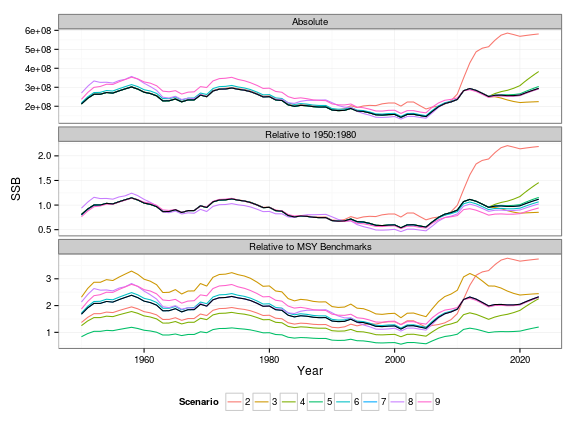
\includegraphics{../figs/om-ssb.png}
\end{center}
\caption{\bf{Time series of SSB for the 9 scenarios, black line is the base case. The panels show the absolute values, values scaled relative to 
the average from the period 1950 to 1980 and values relative to $B_{MSY}$}}
\label{map}\end{figure} 

\begin{figure}[!ht]\begin{center} 
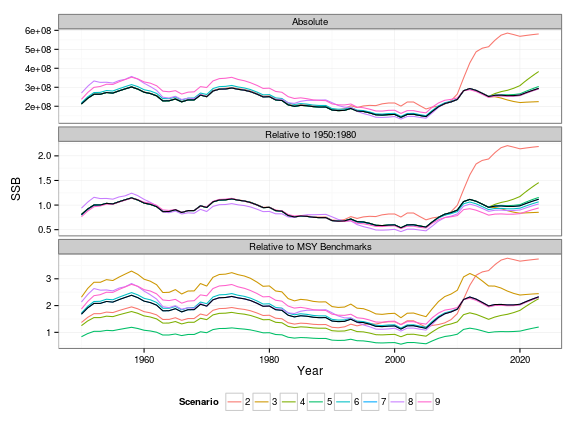
\includegraphics{../figs/om-ssb.png}
\end{center}
\caption{\bf{Time series of SSB for the 9 scenarios, black line is the base case. The panels show the absolute values, values scaled relative to 
the average from the period 1950 to 1980 and values relative to $B_{MSY}$}}
\label{ts-ssb}\end{figure} 


\begin{figure}[!ht]\begin{center} 
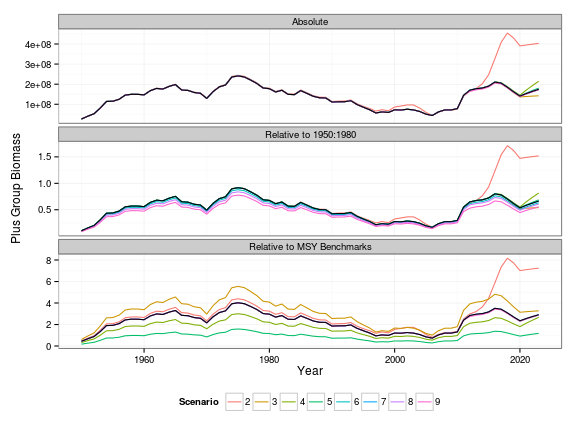
\includegraphics{../figs/om-pg.png}
\end{center}
\caption{\bf{Time series of plus group biomass for the 9 scenarios, black line is the base case. The panels show the absolute values, values scaled relative to 
the average from the period 1950 to 1980 and values relative to plus group biomass at $B_{MSY}$}}
\label{ts-pg}\end{figure} 

\begin{figure}[!ht]\begin{center} 
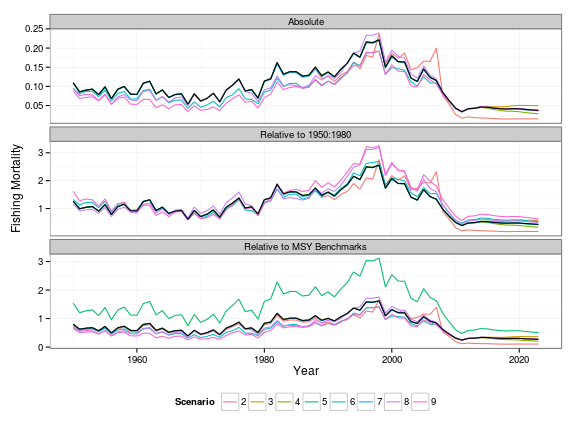
\includegraphics{../figs/om-f.png}
\end{center}
\caption{\bf{Time series of fishing mortality for the 9 scenarios, black line is the base case. The panels show the absolute values, values scaled relative to 
the average from the period 1950 to 1980 and values relative to $F_{MSY}$}}
\label{ts-f}\end{figure} 


\begin{figure}[!ht]\begin{center} 
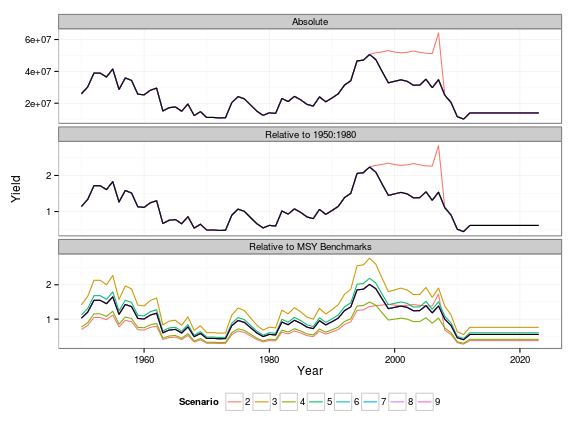
\includegraphics{../figs/om-yield.png}
\end{center}
\caption{\bf{Time series of yield for the 9 scenarios, black line is the base case. The panels show the absolute values, values scaled relative to 
the average from the period 1950 to 1980 and values relative to $MSY$}}
\label{ts-yield}\end{figure} 

\end{document}